\section{M-step}

The article miss at providing a full understanding on how Radial basis functions are used to compute exactly the M-step. In order to implement safely, it is of interest to write down all the analytic computations. So let's start from the beginning:\\

At iteration $k$, in the M-step, we assume that states $(x_t, x_{t+1})$ and the joint state and output $(y_t, y_{t+1})$ follow the laws:
\begin{align*}
  \left[ \begin{array}{c} x_{t}\\ x_{t+1}\\ \end{array} \right] &\sim
    \mathcal{N}\left(
      \left[ \begin{array}{c} \hat{x}_{t|T}\\ \hat{x}_{t+1|T}\\ \end{array} \right],
      \left[ \begin{array}{cc} \hat{P}_{t|T} & \hat{P}_{t,t+1|T}\\ \hat{P}_{t,t+1|T} & \hat{P}_{t+1|T}\\ \end{array} \right]
    \right),
    t=1 \ldots T-1\\
  \left[ \begin{array}{c} x_{t}\\ y_{t}\\ \end{array} \right] &\sim
    \mathcal{N}\left(
      \left[ \begin{array}{c} \hat{x}_{t|T}\\  f(\hat{x}_{t|T}, u_t)\\ \end{array} \right],
      \left[ \begin{array}{cc} \hat{P}_{t|T} & TODO \\ TODO & TODO\\ \end{array} \right]
    \right),
    t=1 \ldots T-1\\
\end{align*}
where the quantities $ \hat{x}_{t|T}, \hat{R}_{t|T}, \hat{P}_{t,t+1|T}$ were computed in the E-step.
So the conditionnal probabilities $(p(x_{t+1} | x_t)$ and $p(y_t | x_t)$ are :
\begin{align*}
  p(x_{t+1} | x_t) &\sim \mathcal{N}\left( \hat{x}_{t+1|T} + \hat{P}_{t+1,t|T}\hat{P}_{t|T}^{-1}\hat{x}_{t|T}, \hat{P}_{t+1|T} +\hat{P}_{t,t+1|T} \hat{P}_{t|T}^{-1} \hat{P}_{t,t+1|T} \right)\\
  p(y_t | x_t) &\sim \mathcal{N}\left( TODO , TODO \right)\\
\end{align*}

Now we want to compute the updated parameter $\theta^{(k)} = (\theta_f^{(k)}, \theta_g^{(k)})$ (and $Q$ and $R$.)\\ 

The updated parameter $\theta^{(k)}$ is the maximizer of the expected complete likelihood :
\begin{align*}
  \theta^{(k)} &= argmax_{\theta}L(\theta)\\
\end{align*}
First we need to express $L(\theta)$ using the graph factorization.
Our graphical model is the following :
\begin{figure}[H]
	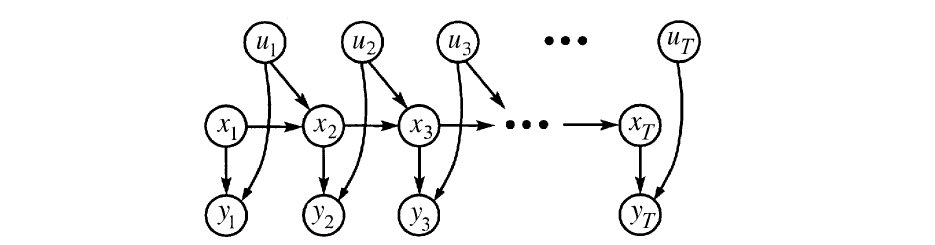
\includegraphics[width=14cm]{screenshot_graphical_model.PNG}
	\captionof{figure}{Graphical model of our system.}
\end{figure}
Firstly, the inputs $u_t$ are not modeled as random variable, so we don't take them into account in the factorization.
Thus, the factorization over the graph yields :
\begin{align*}
p_{\theta}(x,y) &= p_{\theta}(x_1) \prod_{t=1}^{T-1}{p_{\theta}(x_{t+1}|x_t)} \prod_{t=1}^{T}{p_{\theta}(y_t|x_t)}\\
\end{align*}
Thus, if we observe the sequence $(\overline{y}_t)$, the ex
\begin{align*}
  p_{\theta}(x,\overline{y}) &= p_{\theta}(x_1) \prod_{t=1}^{T-1}{p_{\theta}(x_{t+1}|x_t)} \prod_{t=1}^{T}{p_{\theta}(\overline{y}_t|x_t)}\\
\end{align*}

Then the expected complete likelihood (over $p_{\theta^{(k-1)}}(x_t)$ and $p_{\theta^{(k-1)}}(x_t,x_{t+1})$) is written as:
\begin{eqnarray}
L=\mathbb{E}_x(\log(p_{\theta}(x_1)))+\sum_{t=1}^{T-1}{\mathbb{E}_x(\log(p_{\theta}(x_{t+1}|x_t,\overline{u}_t)))}+\sum_{t=1}^{T}{\mathbb{E}_x(\log(p_{\theta}(\overline{y}_t|x_t,\overline{u}_t)))}\nonumber
\end{eqnarray}
\textbf{We want to maximize L and it is separable on $(\theta_f,Q)$, $(\theta_g,R)$}.\\

Section 6.2.3 explains how to maximize each $\mathbb{E}_x(\log(p_{\theta}(\overline{y}_t,x_t)))$ over $(\theta_g,R)$ (situation (3) with j=1) and $\mathbb{E}_x(\log(p_{\theta}(x_{t+1},x_t)))$ over $(\theta_f,Q)$ (situation (1) with j=1).\\
Introducing the author notations (it is the same for $g$, just replace $f$ by $g$): 
\begin{align*}
\theta_f & \overset{\Delta}{=} [h_1^f, \ldots, h_I^f, A^f, B^f, b^f] \\
\Phi_f & \overset{\Delta}{=} [\rho_1^f(x),\ldots, \rho_I^f(x), x^T, u^T, 1]^T \quad\text{(always fixed)} 
\end{align*}
we are able to obtain close form for the optimal parameters in the M-step :

\begin{eqnarray}
(\hat{\theta}_f,\hat{Q})&=&\underset{\theta_f,Q}{\text{argmin }}{\left(\sum_{t=1}^{T-1}{
<(x_{t+1}-\theta_f\Phi_f)^T Q^{-1}(x_{t+1}-\theta_f\Phi_f) >_{x_{t+1},x_t}+\log(|Q|)
}\right)}\nonumber\\
(\hat{\theta}_g,\hat{R})&=&\underset{\theta_g,R}{\text{argmin }}{\left(\sum_{t=1}^{T}{
<(y_{t}-\theta_g\Phi_g)^T R^{-1}(y_{t}-\theta_g\Phi_g) >_{y_t,x_t}+\log(|R|)
}\right)}\nonumber\\
%\hat{\pi}&=& \underset{\pi}{\text{argmax }}{\mathbb{E}_x(\log(p_{\theta}(x_1)))}\nonumber
\end{eqnarray}

Which leads to:
\begin{eqnarray}
\hat{\theta}_f&=&(\sum_{t=1}^{T-1}{<x_{t+1}\Phi_f^T >_{(x_t,x_{t+1})_{old}}})(\sum_{t=1}^{T-1}{<\Phi_f\Phi_f^T >_{(x_t,x_{t+1})_{old}}})^{-1}\\
\hat{\theta}_g&=&(\sum_{t=1}^{T}{<y_{t}\Phi_g^T >_{(x_t)_{old}}})(\sum_{t=1}^{T}{<\Phi_g\Phi_g^T >_{(x_t)_{old}}})^{-1}
\end{eqnarray}

Note that implicitly,for $f$ and $g$, $\Phi=\Phi(x_t)$.

